\chapter{Introduction}

\section{Motivation}
A survey report (\acrshort{nmvccs}) presented by the  U.S. Department of Transportation, National Highway Traffic Safety Administration in 2008 \parencite{nmvccs} shows that about \(94\%\) of road accidents are caused by human errors. Failure to use a seatbelt, excessive speeding, distractions from various sources, and tailgating are among the causes of road incidents. False assumptions about other drivers' habits and neglecting to check traffic before pulling out also contribute to these incidents. With the goal of preventing collisions, cutting emissions, assisting the mobility-impaired in getting around, and easing the stress associated with driving, \acrfull{had} Systems are being researched. The development of deep learning and the accessibility of sensors such as LiDAR, radar, camera, etc have led to significant advancements in computer vision and accelerated the study and application of \acrshort{had} in industry. Autonomous robotaxis are operating in major cities like San Francisco, Phoenix, Beijing, Shanghai, etc \parencite{robotaxis}. Among the sensors such as camera, ultrasonic, radar, and LiDAR, the depth information is captured by all the sensors except camera. Among the depth information capturing sensors, LiDAR has the highest accuracy for a range less than 200 meters \parencite{Yurtsever_2020}. Some features of LiDAR include high depth perception accuracy and resolution, sturdy under dim light, and capable of velocity measurement, etc. However, companies have different carlines and the setup for each carline is different. For detection in short to middle range, cameras are dominantly being used (e.g. Tesla Carlines, Mercedes Class S) in the \acrshort{had} industry. LiDAR and Radar are used in carlines mostly for middle to long-range detection. A LiDAR-equipped Lexus and a Tesla Model 3 were tested in the dark by Luminar to demonstrate the variations in safety measures \parencite{tesla_vs_lexus}. They encountered a dummy pedestrian. The Tesla mowed down the dummy while the Lexus stopped in time. While the system's usefulness cannot be disputed, this seems to indicate that the camera-equipped Tesla is less effective at night. The 2007 DARPA Grand Challenge showcased the capabilities of LiDAR perception systems and was a significant event in the field of autonomous driving. Each of the top three teams' systems was harnessed with LiDAR. Since 2015 \parencite{guo2020deep}, deep learning-based point cloud analysis, including object categorization and segmentation, has advanced significantly thanks to the availability of publically available datasets and progress in deep learning methodology for 3D. Deep learning on 3D \acrshort{pcd}s is still beset by a number of serious difficulties, including the chaotic structure of 3D point clouds, the high dimensionality, and the small size of datasets \parencite{qi2017pointnet}. In the context of LiDAR sensors like Velodyne HDL-64E, the sensor reads more than 1.3 million points per second from space giving an output of 100MBPS UDP Packets \parencite{velodyne_64}. Annotating and verifying each and every point of the LiDAR point cloud is time-consuming. It took annotators about 1700 hours to label and verify the labeling process in the SemanticKITTI dataset \parencite{behley2019semantickitti}.

\begin{figure}[htbp]
    \centering
    \includegraphics[width=0.8\linewidth]{97_graphics//introduction/naturalness_vs_density.pdf}
    \caption{Images from KITTI Vision Benchmark Suite \parencite{Geiger2012CVPR}}
    \label{fig:introduction_surf_variation_in_kitti}
\end{figure}
The distribution of points in the LiDAR point cloud exhibits a notable imbalance between foreground and background elements. Analysis of the KITTI training dataset reveals an average of 19,047 points per scene within the camera's field of view, with approximately 1,382 points (about \(7.25\%\)) falling within 3D bounding box annotations, indicating foreground objects. Similarly, examination of the KITTI validation set shows an average of 18,888 points per scene in the camera field of view, with around 1,641 points (approximately \(8.69\%\)) classified as foreground within 3D bounding box annotations \parencite{DBLP:journals/corr/abs-2004-01643}. This observation highlights a class imbalance between foreground objects and the background scene. According to \parencite{DBLP:journals/corr/abs-1708-02002}, class imbalance poses several challenges. Training efficiency is compromised as a majority of locations represent easy negatives, providing minimal learning signals. The prevalence of these easy negatives can dominate the training process, resulting in the development of degenerate models.
Figure \ref{fig:introduction_surf_variation_in_kitti}, shows a brief look into the diversity of data in SemanticKITTI. It is understood from the figure that most of the data in SemanticKITTI represents either downtown or natural vegetation. So there lies a question of how to close the gap in \acrfull{sota} datasets like SemanticKITTI that is used as a base for semantic understanding of \acrshort{had} system benchmarking \parencite{papers-with-code}. Because of the interactions between vehicles driven by humans, the chances of accidents are low. As a result, the dataset collected in an open-world environment may not represent complete possible scenarios. Such conditions lead to faulty tests of \acrshort{had} systems. For example in 2022, Cruise Robotaxis had 546,492 driverless miles in California and even though the number of miles driven by the autonomous vehicles of Cruise in California for 2023 was a total of 583,624 Miles with 510 Vehicles \parencite{disengagement_report}, accident occurred on February 10, 2023. A woman was struck by a human-driven Nissan at a red light, which caused her to fall under the passenger side of the autonomous Cruise Robotaxi that was moving parallel to the Nissan. When the cab attempted to pull over to the edge of the road, it dragged the woman a few meters instead of stopping instantly \parencite{cruise_crash}. Even though the Cruise Robotaxis had driven millions of miles in the real world as \acrshort{had} system, such a horrific situation occurred due to the result of a scenario that was never seen by the Cruise Robotaxis. Deficits of the variety of scenarios (positions, behavior or pose, the appearance of pedestrians, and also the scenery like the background or surroundings of pedestrians) necessitate a new method of scenario generation that represents the authentic world better than the synthetic simulations and can be employed to evaluate the \acrshort{had} systems effectiveness and harmlessness.

\section{Applications}
Annotated data is necessary to apply deep learning technology. Deep neural network models are trained, validated, and tested using the known labels. A predominant strategy for mitigating the workload associated with data annotation involves the generation of synthetic data through environmental simulations. This approach exhibits potential by streamlining the acquisition of all ground-truth labels. Even though the performance of the object detection models is improved \parencite{johnsonroberson2017driving}, there still exists a domain disparity among the simulated and real-world data \parencite{care_real_and_syn_gap}. There exists a question about the fidelity of sensors in a simulation involving LiDAR because of reasons such as unreturned pulses, multiple echos from the environment, retroreflectors, spurious returns, etc \parencite{zero_domain_gap}. As a result of these factors, achieving high-fidelity modeling of simulators involving LiDAR sensors remains unattained. These factors have prompted the utilization of simulations, such as \acrfull{mil}, \acrfull{sil}, \acrfull{hil}, \acrfull{vil}, etc during the early phases of \acrshort{had} system development and research \parencite{x_in_loop}. Another strategy to deal with limited annotated data is data augmentation \parencite{lidar_aug}. We ask the research question : 
\begin{itemize}
    \item How to address the class imbalance issue i.e. between foreground objects and background scene?
    \item How to mitigate the deficiency in scenarios in the context of \acrshort{had}?
\end{itemize}

\section{Contributions}

This thesis outlines a methodology for generating concrete scenarios utilizing available LiDAR data. Unlike approaches that operate at a higher level, such as simulation, for scenario generation and testing, this research emphasizes a lower-level approach, specifically augmenting point clouds through LiDAR augmentation techniques.

\begin{figure}[htbp]
    \centering
    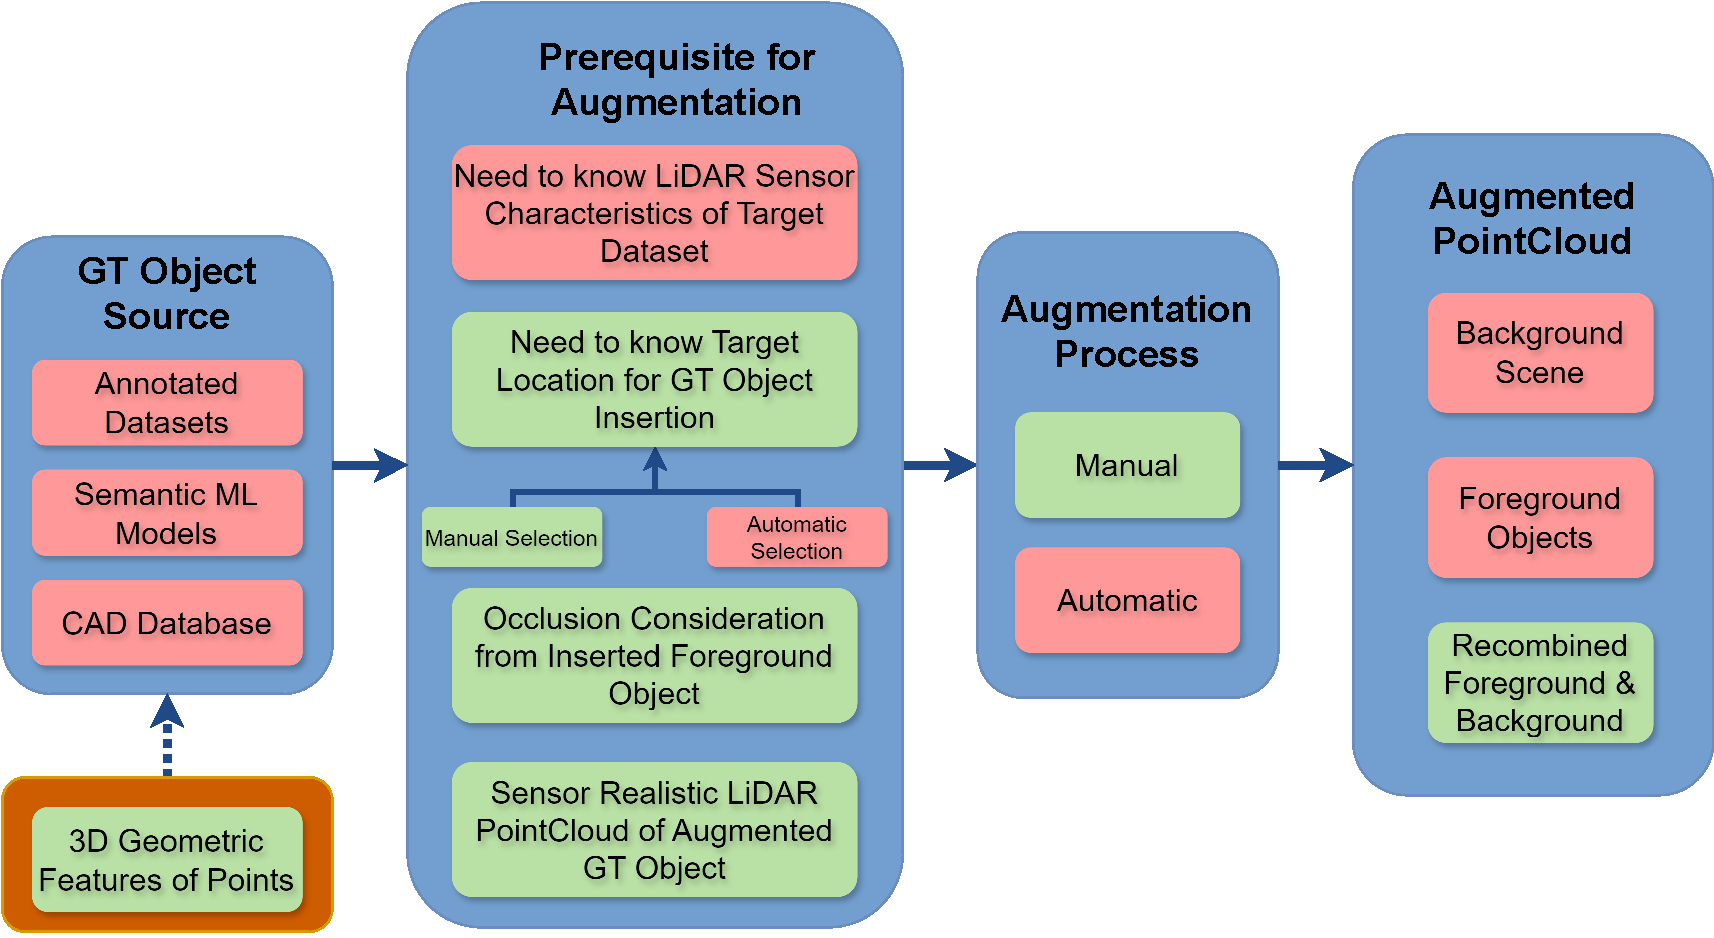
\includegraphics[width=1\linewidth]{97_graphics//related_work/related_work_block_diagram.pdf}
    \caption{Augmentation process of LiDAR Point Cloud.}
    \label{fig:sota-related_work_block_diagram}
\end{figure}


Figure \ref{fig:sota-related_work_block_diagram} illustrates current methods employed in augmenting LiDAR \acrfull{pcd}, where blue-colored blocks represent existing techniques. These methods predominantly rely on annotated datasets, Semantic ML models, or pre-existing CAD models for extracting \acrfull{gt} objects (foreground objects), as indicated by the red-colored blocks within the "GT Object Source" block. The green-colored blocks in the figure signify the approaches adopted in this thesis for scenario generation. Regardless of certain augmentation methods \parencite{9811816, dada_2023}, this thesis does not require prior knowledge of the characteristics of the LiDAR in the target dataset to be augmented. Instead, it leverages the distribution of the target point cloud in the augmentation process to accommodate these characteristics. A distinctive contribution of this work involves leveraging 3D geometric features of points within a local neighborhood for the extraction of ground truth objects from a scene, depicted by the dark orange-colored block on the far left side in figure \ref{fig:sota-related_work_block_diagram}. Implementing this method has the potential to enhance dataset diversity by injecting foreground point cloud objects into scenarios lacking foreground elements, thus addressing the class imbalance issue. Importantly, this approach eliminates the necessity for collecting and annotating new LiDAR data for scenario generation.
